\documentclass[10pt]{article}
\usepackage[preprint]{tmlr}
\usepackage{amsmath,amssymb,booktabs,graphicx,array,longtable,xcolor}
\usepackage{tikz}
\usetikzlibrary{arrows.meta,positioning}
\usepackage{hyperref}
\hypersetup{colorlinks=true,linkcolor=blue!55!black,citecolor=blue!55!black,urlcolor=blue!55!black}
\newcommand{\cka}{\operatorname{CKA}}
\newcommand{\wt}{\operatorname{wt}}
\newcommand{\Ftwo}{\mathbb F_2}
\newcolumntype{L}[1]{>{\raggedright\arraybackslash}p{#1}}
\newcommand{\workshopplaceholder}{\par\noindent\textit{Draft citation note: add the additional workshop paper requested for third-person citation once its title, authors, and venue are verified. The available source index does not uniquely identify that item.}}
\title{When Do Mathematical Correspondences Show Up in Representational Similarity?\\A Controlled Study}
\author{\name Anonymous authors}

\begin{document}
\maketitle
\begin{center}\small Working draft, 12 October 2026. Based on existing exploratory experiments.\end{center}

\begin{abstract}
Exact relationships between mathematical tasks offer a way to ask what a
representational-similarity comparison identifies. We study single-task
specialists on permutation statistics, directed-graph degrees, and binary
matrix statistics. Two comparisons answer different questions: fixing the
task pair while changing the input transformation, and fixing the
transformation while changing the candidate task. In the primary PermWorld
analysis, joint-answer-controlled final-layer CKA favors the correct over the
specified wrong pairing in 26 of 32 conditions. The designated task exceeds
the mean of 14 non-designated candidates in 29 of 32 conditions, but ranks
uniquely first among 15 candidates in 19. Trained preference and change from
initialization are distinct: only 18 conditions have a positive
trained-minus-initial preference increment. Shared initial weights give the
raw fixed-transformation task contrast a zero initialization reference, while
candidate-specific answer stratification does not. A GRU task pair with near-perfect held-out accuracy illustrates how changing the encoding can reverse the increment
without reversing trained preference. Graph and two independently sampled
matrix worlds reveal further control and metric dependence; a matrix
transpose pair with perfect measured task accuracy has negative
size-averaged, answer-controlled CKA preference but
positive neighborhood and Procrustes contrasts. These exploratory findings
support correspondence-associated geometric selectivity under specified
conditions, rather than a universal or uniquely mathematical mechanism. They
also motivate reporting initialization, both pairing contrasts, answer
controls, and prescribed measurement sensitivities together.
\end{abstract}

\section{Introduction}
Representational similarity is often used to argue that neural networks have
learned a common underlying structure. A large similarity value, however,
can reflect several different sources: the inputs used to measure it,
features already present at initialization, properties of the output task,
or a training-dependent organization of hidden states. This ambiguity is
especially relevant when the proposed shared structure is a mathematical
relationship between tasks. If two answers become equivalent after an exact
input transformation, does the same transformation also produce a
distinctive correspondence between their learned representations?

We investigate this question using tasks with explicitly checkable formulas.
For example, the number of descents of a permutation equals the number of
inverse descents of its inverse. Such identities identify a designated task
pair and a correct transformation without selecting them from a similarity
plot. They do not, by themselves, predict that two learned hidden spaces
must become identical, or that every similarity measure must favor the
designated relationship. The tasks may have different difficulty, the input
encoding may make one transformation easier to express than another, and the
same output identity may appear in several kinds of hidden geometry.

Our main study, PermWorld, uses sixteen permutation-statistic specialists,
organized into eight directed correspondences. We compare one-line and
canonical-cycle encodings within two existing model configurations, a
Transformer and a GRU. Each configuration uses saved, genuinely shared
initial weights and a fixed training endpoint. We also examine a small
directed-graph study and two independently sampled binary-matrix worlds.
These additional settings delimit the observation; their different task
families and sampling distributions do not form a controlled domain
intervention.

The central distinction is between two comparisons. First, a correct
transformation can produce more similar representations than a specified
wrong transformation for the same two models. Second, under a fixed
transformation, the designated task model can be more similar than models
trained for other tasks. Neither comparison implies the other. Nor does a
positive preference after training imply a positive change from
initialization. We keep these quantities separate throughout the study.

The paper makes three contributions:
\begin{enumerate}
\item A paired measurement design separating input-pairing selectivity from
task-candidate selectivity, with an explicit shared-initialization reference
and a decomposition of training increments into correct and wrong scores.
\item A complete exploratory PermWorld grid showing both the extent and the
limits of correspondence-associated selectivity across encodings,
configurations, layers, and controls. We report both above-mean and first-rank
candidate counts, retaining all negative conditions.
\item Cross-system examples that show why answer controls and alternative
readouts matter even when source tasks are well learned, together with
concrete guidance for similarity-based arguments about shared structure.
\end{enumerate}
Our claim concerns measured geometric preferences. We do not use these
measurements to identify an internal mathematical algorithm or establish a
functional transfer benefit.

\section{Related work}
\label{sec:related_work}

\paragraph{Task similarity and task taxonomies.}
Relationships between training objectives provide an established explanation for
representational similarity. \citet{li2025causes} manipulate dataset and task
overlap, finding greater similarity with greater overlap across several model
settings. Their constant-data experiment changes the labeling of identical
images to separate task overlap from shared examples.
\citet{dwivedi2019rsa} use representational similarity analysis between visual
task models to construct a task taxonomy and examine associations with transfer
performance. These studies motivate examining how task definitions shape
geometry. The present study examines single-task specialists with exactly
specified mathematical correspondences. One comparison fixes both specialists
and changes the input pairing among correct, originally specified wrong, and
identity transformations. A second fixes the left specialist, transformation,
and anchors while varying the right task. Together, these comparisons ask where
a designated correspondence has a geometric preference relative to explicit
input-pairing and task-candidate comparators.

\paragraph{Representational convergence.}
\citet{huh2024platonic} propose the Platonic Representation Hypothesis and report
increasing agreement between vision and language representations with model
scale. \citet{park2026convergent} study geometric tasks over a shared world of
city coordinates. Multi-task training aligns representations even for
non-overlapping task sets, while some tasks impair the integration of new
entities through fine-tuning. This distinction between aligned geometry and
adaptability is relevant here. The current experiments preserve individual
correct and wrong scores, trained pairing preferences, and initialization
preferences, so that an increment can be distinguished from an increase in
correct-pair similarity. Their scope is exploratory correspondence-associated
geometry; functional benefit requires separate evidence.

\paragraph{Grounding and calibrating similarity measurements.}
CKA supplies invariances useful for comparing representations
\citep{kornblith2019}, but a similarity value requires an appropriate reference.
The ReSi benchmark evaluates measures using prediction-grounded and
design-grounded tests, reflecting multiple meanings of model similarity
\citep{klabunde2025resi}. \citet{cui2022deconfounded} show that input population
structure can inflate RSA and CKA, including comparisons of random networks,
and propose covariate-adjustment regression.
\citet{groger2026aristotelian} identify model-scale confounding and introduce
permutation-null calibration, separating global spectral convergence from
local neighborhood agreement. These results motivate retaining input,
initialization, answer, and output references and checking prescribed
alternative metrics. The present trained-minus-initial preference contrast has
its own definition and is distinct from permutation calibration. Answer
stratification also retains pair-specific supports and cannot remove every
confidence or nonlinear answer contribution. No subtraction of hidden and
output scores is interpreted as an isolated internal mechanism.

\paragraph{Permutation encodings and preceding work.}
\citet{scullen2025permutations} use permutation statistics to study how encoding,
data availability, and MLP or Transformer models affect learning. Their five
encodings comprise permutation matrices, inversion vectors, Lehmer cocodes,
major codes, and lexicographically minimal reduced words. They identify internal-representation comparison
as a direction for further study. The present one-line and canonical-cycle
encodings support an additional comparison of initialization and trained
pairing preferences, with all declared layers and relations retained. Model
capacity and task proficiency differ across configurations, limiting a pure
architecture interpretation. The GraphWorld and MatrixGroupWorld analyses
examine the scope of the same comparisons in additional mathematical settings,
with their negative, undefined, and failed verification results preserved.

\workshopplaceholder


\section{Study design and two distinct comparisons}
\label{sec:design}
\subsection{What each comparison answers}
Let $f$ be a left task, $g_*$ its designated right task, and $T$ an input
transformation. A relation has the form
\begin{equation}
 f(x)=\phi\bigl(g_*(T(x))\bigr),
 \label{eq:identity}
\end{equation}
where $\phi$ is a specified answer-coordinate map. It is the identity for most
PermWorld relations, a shift for one permutation relation, and a complement
map for graph-degree complement relations. These formulas are verified
against the task generators. They are specified independently of the
geometric scores.

\textbf{Comparison A: fix the two tasks, change the input pairing.}
We compare $h_f(x)$ with $h_{g_*}(T(x))$ and with
$h_{g_*}(U(x))$, where $U$ is the original specified wrong transformation.
The question is whether the designated transformation is preferred over
that comparator for these same two trained specialists. The identity
pairing is also retained. A wrong transformation need not break the
answer identity on every input.

\textbf{Comparison B: fix the input transformation, change the right task.}
We instead keep the left model, $x$, and $T(x)$ fixed and compare
$h_f(x)$ with $h_g(T(x))$ for every available $g\ne f$.
The question is whether $g_*$ stands out among candidate task models under
the same input transformation. In PermWorld this gives fifteen candidates,
including the designated task, and fourteen non-designated comparators.
GraphWorld and MatrixGroupWorld each give three candidates. A
non-designated task is not asserted to lack all mathematical relationships
with $f$. Task identity, output statistics, and proficiency also differ
between these candidates.

\begin{figure}[t]
\centering
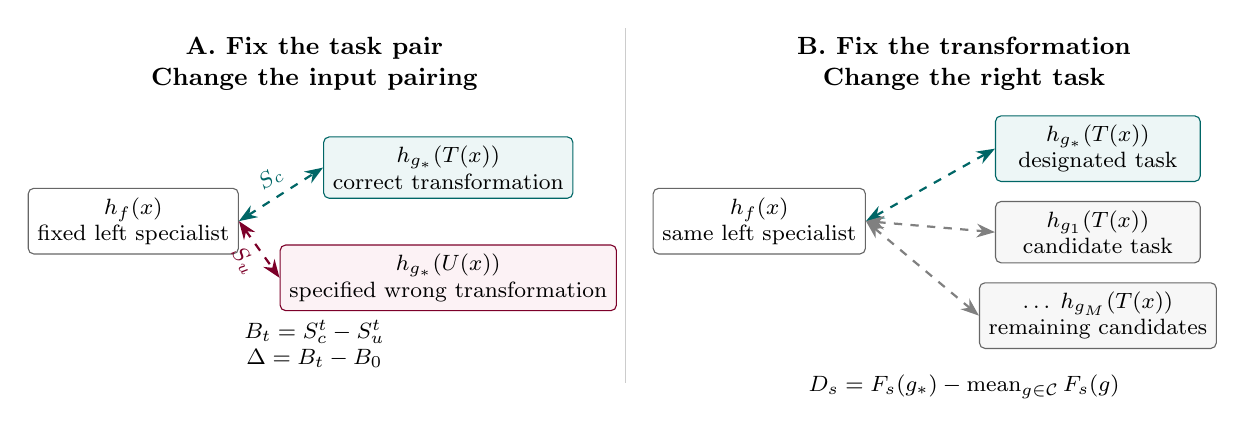
\begin{tikzpicture}[x=1cm,y=1cm,font=\footnotesize,
  state/.style={draw=black!60,rounded corners=2pt,minimum height=.65cm,align=center},
  designated/.style={state,draw=teal!80!black,fill=teal!7},
  compare/.style={<->,dashed,>=Stealth,thick}]
\node[align=center,font=\small\bfseries] at (3.45,3.5)
  {A. Fix the task pair\\Change the input pairing};
\node[state,minimum width=2cm] (lefta) at (1.15,1.5) {$h_f(x)$\\fixed left specialist};
\node[designated,minimum width=2.9cm] (correcta) at (5.15,2.18) {$h_{g_*}(T(x))$\\correct transformation};
\node[state,draw=purple!65!black,fill=purple!5,minimum width=2.9cm] (wronga) at (5.15,.78) {$h_{g_*}(U(x))$\\specified wrong transformation};
\draw[compare,teal!80!black] (lefta.east) -- node[above,sloped] {$S_c$} (correcta.west);
\draw[compare,purple!65!black] (lefta.east) -- node[below,sloped] {$S_u$} (wronga.west);
\node[align=center] at (3.45,-.06) {$B_t=S_c^t-S_u^t$\\$\Delta=B_t-B_0$};
\draw[black!20] (7.4,-.55)--(7.4,3.95);
\node[align=center,font=\small\bfseries] at (11.7,3.5)
  {B. Fix the transformation\\Change the right task};
\node[state,minimum width=1.8cm] (leftb) at (9.1,1.5) {$h_f(x)$\\same left specialist};
\node[designated,minimum width=2.6cm] (correctb) at (13.4,2.42) {$h_{g_*}(T(x))$\\designated task};
\node[state,minimum width=2.6cm,fill=black!3] (otherb) at (13.4,1.36) {$h_{g_1}(T(x))$\\candidate task};
\node[state,minimum width=2.6cm,fill=black!3] (lastb) at (13.4,.30) {$\ldots\;h_{g_M}(T(x))$\\remaining candidates};
\draw[compare,teal!80!black] (leftb.east)--(correctb.west);
\draw[compare,black!50] (leftb.east)--(otherb.west);
\draw[compare,black!50] (leftb.east)--(lastb.west);
\node[align=center] at (11.7,-.60) {$D_s=F_s(g_*)-\operatorname{mean}_{g\in\mathcal C}F_s(g)$};
\end{tikzpicture}

\caption{Two comparisons with different fixed factors. Left: the same pair
of specialists is evaluated under the correct $T$ and specified wrong $U$;
$B_t$ contrasts these two similarities. Right: the input transformation
stays $T$ while the right task varies; $D_t$ contrasts the designated
specialist with a prespecified candidate category. Dashed links denote
similarity comparisons, not learned computational mappings. All states are
taken before the task token. Shared initial weights give the \emph{raw}
right-hand contrast a zero reference; candidate-specific answer controls
can change that reference.}
\label{fig:comparisons}
\end{figure}

\subsection{Scores, preferences, and training increments}
For Comparison A, with $s\in\{0,t\}$ denoting saved initialization and the
fixed trained endpoint, define
\begin{align}
 S_c^s &= S\bigl(h_f^s(x),h_{g_*}^s(T(x))\bigr), &
 S_u^s &= S\bigl(h_f^s(x),h_{g_*}^s(U(x))\bigr),\nonumber\\
 B_0 &= S_c^0-S_u^0, & B_t&=S_c^t-S_u^t,\label{eq:preferences}\\
 \delta_c &= S_c^t-S_c^0, & \delta_u&=S_u^t-S_u^0,\nonumber\\
 \Delta &=B_t-B_0=\delta_c-\delta_u.\label{eq:increment}
\end{align}
We preserve the four original scores as well as these contrasts. Positive
$\Delta$ can come from a reduction of wrong-pair similarity without an
increase of correct-pair similarity. Changing an initialization reference
changes $\Delta$, not an already fixed $B_t$.

For Comparison B, use separate notation,
\begin{equation}
 F_s(g)=S\bigl(h_f^s(x),h_g^s(T(x))\bigr),\qquad
 D_s=F_s(g_*)-\frac{1}{|\mathcal C_s^{\rm fin}|}\sum_{g\in\mathcal C_s^{\rm fin}}F_s(g),
 \label{eq:taskcontrast}
\end{equation}
where $\mathcal C$ is the prespecified comparator category and
$\mathcal C_s^{\rm fin}$ its finite, complete-length candidates at phase
$s$. The contrast is undefined if the designated score is undefined or this
set is empty. We report every candidate and all finite/undefined counts.
In the main PermWorld grid, all fifteen candidates are finite in both
phases. An optional training change recomputes both means on the common
set $\mathcal C_0^{\rm fin}\cap\mathcal C_t^{\rm fin}$; it is a different
contrast from $\Delta$ in Eq.~\ref{eq:increment}.

The primary score is ordinary linear CKA \citep{kornblith2019}. For centered
sample-by-feature matrices $X$ and $Y$,
\begin{equation}
 \cka(X,Y)=\frac{\|X^\top Y\|_F^2}
 {\|X^\top X\|_F\,\|Y^\top Y\|_F}.
\end{equation}
Zero-variance or otherwise undefined measurements remain undefined. The
other final-layer readouts are ten-neighbor overlap and negative held-out
normalized Procrustes error; their larger-is-more-similar convention is
fixed, but their scales and normalizations differ. They are sensitivities on the same
representations, not independent replications or functional measurements.

\subsection{Shared initialization and its exact scope}
\label{sec:sharedinit}
Within a PermWorld architecture, all sixteen specialists and both encodings
start from \emph{the same numerical initial parameters}, copied from a
saved step-0 state. This is stronger than reusing a seed. Checkpoint and
parameter hashes bind the initial identities, including the recorded
value-preserving GRU key conversion. GraphWorld copies the same saved
Transformer initialization used in PermWorld. In MatrixGroupWorld the four
specialists within each of two units share that unit's saved initial
weights; the units themselves use independently sampled data and initials.

The measurement point is the end of the encoded input, before the task
token, with models in evaluation mode and dropout disabled. Therefore,
under shared weights, a right specialist's \emph{raw}
initial state at $T(x)$ is independent of its eventual task $g$. With a
common anchor set and task-independent preprocessing, and when $S$ is
defined and the comparator category is nonempty,
\begin{equation}
 h_g^0(T(x))=h_0(T(x))\quad\Longrightarrow\quad
 F_0(g)=F_0(g')\quad\Longrightarrow\quad D_0=0.
 \label{eq:initialnull}
\end{equation}
Consequently the raw fixed-transform task preference in this design arises
after training. This statement does not isolate the mathematical relation
from other effects of task training. It also does not apply to
task-conditioned outputs, or to answer-controlled scores with
candidate-specific residualization.

For Comparison A the correct and wrong inputs already differ at step 0;
$B_0$ is generally nonzero even though the models share weights. These
different initialization references explain why the two comparisons give
different answers to ``did the preference emerge through training?''

\subsection{Systems, training, and coverage}
\label{sec:coverage}
Table~\ref{tab:coverage} separates model coverage from independent sampled
units. PermWorld supplies sixteen statistics and eight exact directed
relations (Appendix~\ref{app:relations}). The two input encodings describe
the same permutations: one-line notation and cycle notation normalized by
cycle rotation and ordering. All elements, including fixed points, are
represented. The two configurations share vocabulary, width 256, four
layers, and dropout 0.1. The Transformer has eight heads and approximately
3.24 million parameters; the GRU has approximately 1.66 million. Their
capacities are not matched.

\begin{table}[t]
\centering\small
\begin{tabular}{L{1.35cm}L{2.25cm}L{3.05cm}L{3.0cm}L{3.25cm}}
\toprule
System & Tasks / trained sources & Configurations and input sizes & Units and initial-weight sharing & Comparison coverage\\
\midrule
Perm & 16 / 64 & Transformer, GRU; two encodings; $n=10,\ldots,30$ & One paired data world; one actual initial per architecture, copied across tasks and encodings & A: $8\times4=32$; B: $32\times15=480$ candidates\\
Graph & 4 / 4 & Transformer; off-diagonal adjacency tokens; $n=6,7,8$ & One world; PermWorld Transformer initial reused & A: 4; B: $4\times3=12$ candidates\\
Matrix & 4 / 8 & Transformer; row-major binary tokens; $n=6,8,10$ & Two independent data/initial units; four tasks share weights within each unit & A: $4\times2=8$; B: $8\times3=24$ candidates\\
\bottomrule
\end{tabular}
\caption{Coverage, rather than independent replication counts. All 76 source
models have actual fixed 20k endpoints. Comparison B uses ordinary final-layer
CKA only. In PermWorld, layer analyses use CKA and its prescribed debiased
sensitivity; the three principal geometric readouts are jointly available
at the final state. Shared tasks, transformations, models, inputs, and
initials create dependence within these grids.}
\label{tab:coverage}
\end{table}

Each task is trained separately to emit an answer token and EOS. No
representation-alignment loss or relation-supervised operator is used.
The common declared budget is 20,000 updates with effective batch size 64,
giving 1,280,000 example exposures per specialist. Endpoints are fixed,
not selected for geometric results or best validation accuracy. Within a
world, data and batch schedules are shared across tasks; encoding pairs
also share their recorded starting random state. Sixteen existing
PermWorld endpoints were reused and forty-eight were completed later with
documented source and engineering-repair histories. These histories are
preserved rather than claiming that all executions used one byte-identical
program revision. Appendix~\ref{app:training} gives optimization and
random-stream details.

All systems use 4,096 training, 256 validation, and 512 held-out anchors per
declared size. Splits follow their documented transform-orbit exclusions.
In PermWorld only accepted eight-element orbits are used; matrices require
exact full rank over $\Ftwo$ and exclusion of overlapping embedded
$\mathrm{GL}(2,\Ftwo)$ action/transpose orbits. These conditional sampling
rules do not imply uniform sampling over all mathematical objects.

\subsection{Controls and aggregation}
\label{sec:controls}
CKA is calculated separately within every size, then aggregated with fixed
weights $1/21$ for PermWorld and $1/3$ for GraphWorld and MatrixGroupWorld.
Subtracting length means and pooling all lengths is not substituted for
this procedure. Any undefined size component leaves its aggregate
undefined; weights are not redistributed.

The primary control subtracts means within joint gold-answer strata. For a
candidate $g$, the key records size, the left identity answer, and mapped
right answers on the identity, correct, and wrong views. A stratum requires
at least three samples separately in the fitting and held-out splits.
The same retained anchors and groups are used across phases and input
roles for a given pair. In Comparison B, changing $g$ changes these labels
and can change both groups and support. Writing its residualization
operator as $R_g$ makes the scope of Eq.~\ref{eq:initialnull} explicit:
\begin{equation}
 F_0^{\rm answer}(g)=
 \cka\bigl(R_gH_0(x),R_gH_0(T(x))\bigr)
 \quad\text{need not be constant in }g.
 \label{eq:residualinit}
\end{equation}
This is a control for between-group answer geometry, not removal of all
answer information, confidence, or prediction-error structure. We retain
true-answer and output-probability baselines, and do not interpret hidden
minus output contrasts as a mechanism estimate. GraphWorld's additional
answer-plus-exact-edge-count control remains a separate sensitivity.

Procrustes maps are fitted only on validation features, with a prescribed
PCA rank cap of eight, RMS scaling, and orthogonal alignment; held-out
features are centered according to the original protocol. Neighbor overlap
uses $k=10$ with stable anchor-ID tie rules and the original duplicate
exclusions. We retain numerical failures and undefined values. The fixed
candidate catalogue distinguishes designated, other-known-exact, and
non-designated correspondences before their scores were evaluated; the
other-known-exact category is empty in the available PermWorld candidate
catalogue, not a proof of absence of other relations.

\section{Results: three questions}
\label{sec:results}
All results below are exploratory. The candidate analysis was frozen before
its scores were computed, after earlier training and geometric results had
been seen. We therefore do not describe it as an independently
preregistered confirmation. Counts summarize coupled conditions; they are
not sample sizes for a binomial test.

\subsection{Question 1: do designated correspondences have geometric selectivity?}
In Comparison A, joint-answer-controlled final-layer ordinary CKA yields
$B_t>0$ in 26 of the 32 PermWorld conditions
(Figure~\ref{fig:permgrid}). The other six conditions are all
canonical-cycle encodings: descents/inverse descents, fixed/anti-fixed
points, and global descents/components for the Transformer; fixed/anti-fixed
points, increasing/decreasing runs, and global descents/components for the
GRU. This concentration is a descriptive encoding association, not evidence
that encoding is the sole cause or that the negative cases are noise.

\begin{figure}[t]
\centering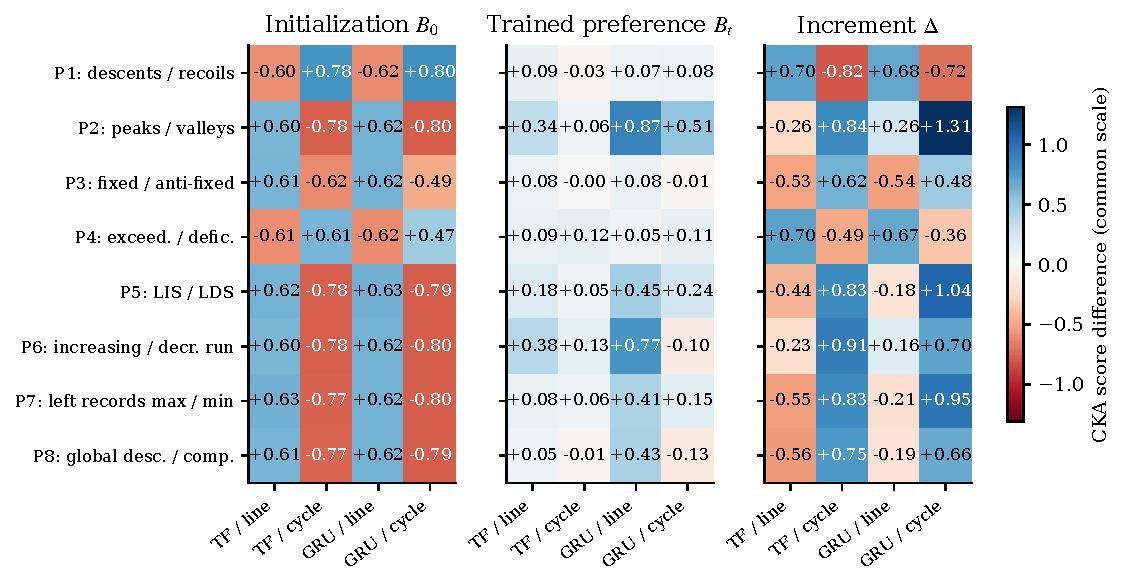
\includegraphics[width=\linewidth]{figures/figure2_perm_preferences.pdf}
\caption{All eight PermWorld relations and four configuration/encoding
conditions under joint-answer control, final normalization, and
equal-within-length ordinary CKA. Initialization preference $B_0$, trained
preference $B_t$, and increment $\Delta$ use a common color scale. Positive
trained preference occurs in 26/32 conditions, but positive increment in
18/32. The raw scores and their correct/wrong changes are retained in
Appendix~\ref{app:fullperm}; task IDs P1--P8 are defined in
Table~\ref{tab:relations}. This figure does not summarize other layers or
controls.}
\label{fig:permgrid}
\end{figure}

Comparison B asks a different task-identification question while holding the
transformed input fixed. Under the same primary answer-controlled readout,
the designated specialist exceeds the mean of the fourteen non-designated
specialists in 29/32 conditions, but is uniquely first among all fifteen
candidates in 19/32 (Figure~\ref{fig:fixedtransform}). All fifteen candidates
are finite in these main conditions. Above-mean preference is therefore
more frequent than uniquely identifying the designated model.
Table~\ref{tab:permcounts} also gives the raw readout, so that this observation
is not tied to reporting only the favorable control.

\begin{table}[t]
\centering\small
\begin{tabular}{lcccc}
\toprule
& \multicolumn{2}{c}{A: vary input pairing} & \multicolumn{2}{c}{B: vary right task}\\
\cmidrule(lr){2-3}\cmidrule(lr){4-5}
Control & $B_t>0$ & $\Delta>0$ & Above other mean & Unique first of 15\\
\midrule
Raw, within length & 27/32 & 25/32 & 30/32 & 25/32\\
Joint-answer strata & 26/32 & 18/32 & 29/32 & 19/32\\
\bottomrule
\end{tabular}
\caption{Different questions and different readouts. The mean in Comparison
B contains fourteen non-designated tasks; the ranking includes the
designated task. All rows use final-layer ordinary CKA and the original
equal 21-length weights. Counts are descriptive, dependent cells.}
\label{tab:permcounts}
\end{table}

For context, if the designated identity were exchangeable among fifteen
untied scores, its chance of ranking first would be $1/15\simeq6.7\%$.
The observed 19/32 ($59.4\%$) is well above this \emph{descriptive reference}.
Task labels, distributions, and learning difficulties are not exchangeable
here, and conditions share models and inputs. We therefore do not attach
a binomial $p$-value or treat $1/15$ as a validated experimental null.

\begin{figure}[p]
\centering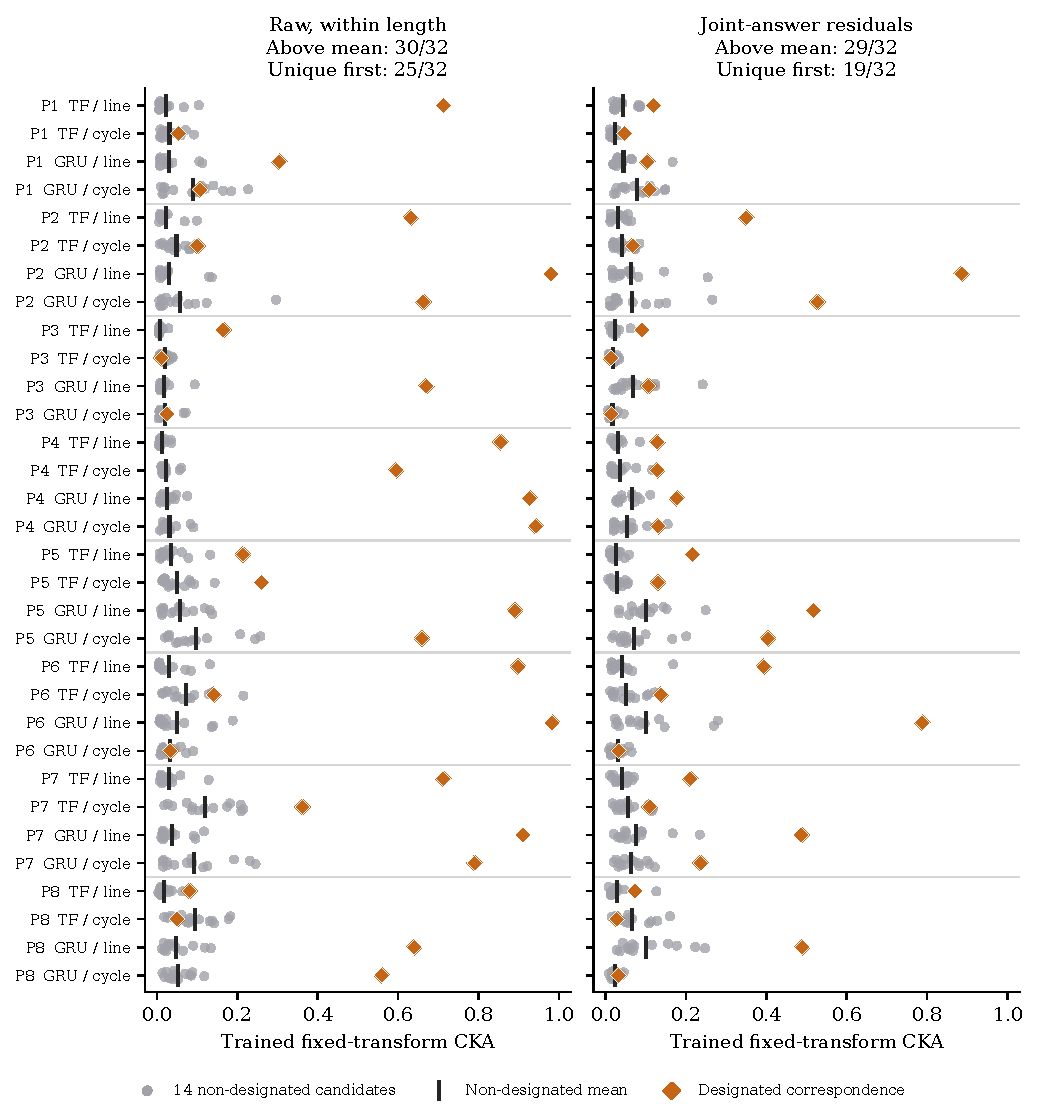
\includegraphics[width=.99\linewidth]{figures/figure3_fixed_transform.pdf}
\caption{Every trained fixed-transform candidate score for the 32 PermWorld
conditions. Each row fixes the left specialist, transformation, input
anchors, encoding, and configuration. Gray points are the fourteen
non-designated specialists, black ticks their mean, and orange diamonds
the designated specialist. Raw and answer-controlled scores are separate.
The latter use candidate-specific strata despite sharing the underlying
anchor pool. Initial raw candidate scores are identical, but initial
answer-controlled candidate scores need not be. Neither these 480 logical
candidate pairings nor the two controls are independent replications.}
\label{fig:fixedtransform}
\end{figure}

\subsection{Question 2: what changed through training, and what changed with encoding?}
The shared-initialization reference answers this question differently for
the two comparisons. In the raw version of Comparison B, candidate initial
scores are identical within every fixed condition; stored designated-minus-
mean contrasts differ from zero by at most $1.4\times10^{-17}$ from mean
summation. Thus raw designated-task advantages arise after the specialists
have been trained. In the answer-controlled version, none of the 32
designated-minus-mean initial contrasts is exactly zero: four are positive
and twenty-eight negative, ranging from $-0.2477$ to $+0.0935$.
This difference is consistent with candidate-specific groups and support,
not a failure of initial-weight identity.

In Comparison A, $B_0$ is already influenced by the geometry of $T$ and
$U$ on each encoding. Accordingly, trained preference is positive in
26/32 conditions while $\Delta$ is positive in only 18/32. A negative
increment does not imply a negative final preference. Conversely, a large
positive increment may be driven primarily by the wrong score decreasing.
For the one-line Transformer descents/inverse-descents pair, correct
answer-controlled CKA changes from $0.0660$ to $0.1191$, while wrong CKA
changes from $0.6709$ to $0.0260$. The resulting $\Delta=0.6980$ contains
a $0.6449$ contribution from the wrong-score decline and only a $0.0531$
correct-score increase. It measures a reshaping of selectivity, not a
$0.6980$ increase of correct-pair agreement.

The GRU exceedances/deficiencies pair supplies a case where weak learning
is not an adequate account of an encoding-dependent increment
(Table~\ref{tab:gruexample}). Both tasks attain approximately 99--100\%
held-out answer accuracy in both encodings. The trained preference stays
positive, increasing from $0.0455$ to $0.1098$, whereas $\Delta$ changes
from $+0.6685$ to $-0.3612$ because $B_0$ changes from $-0.6230$ to
$+0.4710$. This is an increment reversal without a reversal of trained
relationship preference.

\begin{table}[t]
\centering\small
\begin{tabular}{lrrrrr}
\toprule
GRU encoding & $B_0$ & $B_t$ & $\Delta$ & Left acc. & Right acc.\\
\midrule
One-line & $-0.6230$ & $+0.0455$ & $+0.6685$ & 99.88\% & 99.30\%\\
Canonical cycle & $+0.4710$ & $+0.1098$ & $-0.3612$ & 100.00\% & 100.00\%\\
\bottomrule
\end{tabular}
\caption{Exceedances/deficiencies, joint-answer-controlled final CKA.
Accuracy is the original equal-length held-out identity-input answer
accuracy over the full vocabulary. Task proficiency is high in both
encodings, yet the initial preference and training increment differ.
The trained preference has the same sign.}
\label{tab:gruexample}
\end{table}

More generally, for an encoding comparison define
$\Gamma_0=B_0^{\rm cycle}-B_0^{\rm line}$ and
$\Gamma_t=B_t^{\rm cycle}-B_t^{\rm line}$. Then
$\Gamma_\Delta=\Gamma_t-\Gamma_0$. Reporting only
$\Gamma_\Delta$ would conflate a change of initialization preference with a
change of trained preference. All thirty-two individual correct and wrong
changes remain available in Appendix~\ref{app:fullperm}.

\subsection{Question 3: which measurement and system dependencies remain?}
\label{sec:dependencies}
\paragraph{Layers and readouts in PermWorld.}
At the primary final state, ordinary CKA, neighbor overlap, and held-out
Procrustes have matching $B_t$ directions in 32/32 conditions and matching
$\Delta$ directions in 30/32. The two increment disagreements are the one-line GRU peaks/valleys and
increasing/decreasing-run pairs: CKA and Procrustes have positive
$\Delta$, but neighbor overlap has negative $\Delta$. Their exact values
are retained in the released tables. These are geometrically different readings of the
same activations, not three independent reproductions.
Multilayer CKA is also not uniformly selective
(Figure~\ref{fig:layers}). For example, the GRU has positive answer-controlled
$B_t$ in 8/16 conditions at layer 1 and 13/16 at layer 4 and final
normalization. The Transformer changes from 10/16 to 13/16.
The input-end embedding score is undefined in all sixteen conditions of
each architecture under this control; it cannot serve as a numerical zero
or a useful measurement of pooled input content. Changes between layer 4
and final normalization reflect normalization, including learned affine
parameters, rather than a fifth Transformer or recurrent block.

\begin{figure}[t]
\centering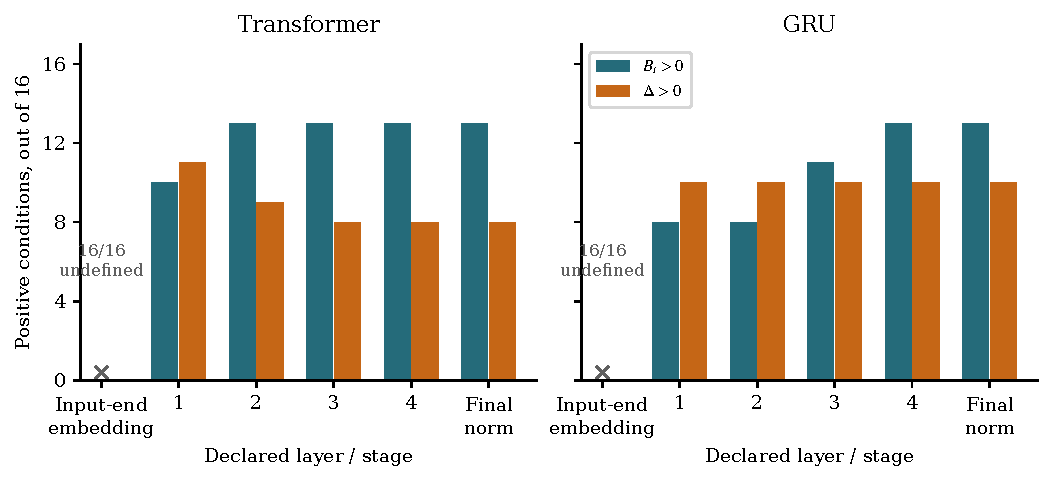
\includegraphics[width=\linewidth]{figures/figure4_layers.pdf}
\caption{Prescribed layer/stage CKA readouts on all eight relations and both
encodings within each architecture: sixteen coupled conditions per panel.
Bars count positive $B_t$ and $\Delta$ under the same answer control and
fixed length weights. Input-end embedding scores are all undefined, not
zero. Neither the most favorable layer nor a different subset is selected
as a new primary analysis. Final-layer kNN/Procrustes agreement is a
separate sensitivity and is not implied for every plotted layer.}
\label{fig:layers}
\end{figure}

\paragraph{Output references.}
The numeric-output probability baseline also contains pairing preferences:
raw ordinary CKA has positive $B_t$ in 29/32 conditions and positive
$\Delta$ in 30/32; after answer control these counts are 29/32 and 16/32.
It is evaluated at a task-conditioned output point, unlike the primary
pre-query hidden state. Gold-answer stratification does not remove all
confidence and prediction-error geometry. These parallel readouts therefore
remain relevant alternative explanations, not quantities that can be
subtracted from hidden scores to estimate an additional mechanism.

\paragraph{Directed graphs and answer structure.}
GraphWorld uses maximum/minimum in- and out-degree specialists and exact
edge-reversal or complement correspondences. Raw final CKA gives positive
$B_t$ and $\Delta$ in all four relations; after joint-answer control,
$B_t$ is positive in two and $\Delta$ in none. The contrast therefore
depends substantially on the measured answer-related geometry.
In Comparison B the raw designated task is uniquely first in all four
relations; under answer control it exceeds the other-task mean in three
and is uniquely first among three candidates in two. These are again
different contrasts, with the full twelve-candidate table retained.
Answer-plus-edge-count stratification is retained as a separate sensitivity;
its changed groups do not automatically make it the uniquely correct
readout. The four original wrong-transform comparators happen to satisfy
their designated answer formulas on 54.8--59.7\% of raw analysis anchors.
These actual-sample rates differ from the earlier random mathematical
audit. We retain those rows and comparators, limiting the claim to the
specified contrast rather than a perfect relation-breaking intervention.
GraphWorld also shares the PermWorld Transformer initial, so it is not
independent initialization replication.

\subsubsection{Independent paired worlds}

MatrixGroupWorld provides two independently resampled worlds, each with new data and a new initialization. Within each world, four task specialists share a saved, genuine initialization and each completes the fixed 20,000-update budget. We report both worlds separately, with equal weights over $n\in\{6,8,10\}$ and the same prespecified transformations, controls, and metrics. These worlds repeat the matrix setting; they do not independently confirm PermWorld across initializations. Because data and initialization vary together, differences between worlds do not isolate a causal effect of initialization. The four relations, three sizes, and three metrics are coupled measurements rather than additional independent replications.

\subsubsection{R1: an illustrative case}

R1 relates $F_1$ and $F_2$ through transposition. Both tasks achieve 100\% full-vocabulary answer accuracy in both worlds at every size on the complete identity training, validation, and analysis sets. The $F_2$ models also achieve 100\% analysis accuracy under the correct and wrong R1 transformations. Nevertheless, their geometric pairing preference depends on the control and metric (Figure~\ref{fig:matrixcase}; Table~\ref{tab:matrix_r1}). This makes R1 an illustrative case, rather than evidence for a general reversal of relation preference.

For raw, size-stratified hidden-state CKA, worlds one and two respectively give $(B_t,\Delta)=(0.520209,0.519581)$ and $(0.558791,0.553006)$. After joint-answer-stratum control, these become $(-0.019384,-0.020747)$ and $(-0.014022,-0.014551)$. Thus, these controlled, equally weighted CKA estimates favor the wrong pairing. Answer control changes both centering and retained sample support; this contrast cannot be interpreted as a causal subtraction of all answer information.

The fixed-transform comparison supplies an additional distinction. For R1,
the designated task ranks uniquely first among three candidates under answer
control in both worlds, both initially and after training. Its advantage over
the two non-designated tasks changes from $0.1894$ to $0.1182$ and from
$0.1179$ to $0.0663$. Thus first rank in Comparison B can coexist with a
negative input-pairing preference in Comparison A, and its controlled task
advantage need not originate at training.

The controlled sensitivity metrics give different aggregate directions. For $k$NN overlap, $(B_t,\Delta)$ is $(0.047718,0.039648)$ and $(0.081837,0.069883)$; for held-out Procrustes it is $(0.052454,0.038940)$ and $(0.045210,0.036150)$. Procrustes is scored as negative alignment error, so larger values indicate better alignment. These metrics use different scales; their numerical magnitudes are not directly comparable. Raw $B_t$ and $\Delta$ are positive for all three metrics in both worlds, whereas controlled CKA disagrees with the two sensitivity metrics. This aggregate disagreement also has size-specific qualifications: controlled CKA has positive $B_t$ and $\Delta$ at $n=10$ in both worlds, while controlled Procrustes has negative $B_t$ and $\Delta$ at $n=6$ in both. World one's controlled $k$NN $B_t$ and $\Delta$ are negative at $n=8$. We retain all sizes rather than select a uniformly positive or negative subset.

R3 illustrates why $\Delta$ must also be decomposed. Its controlled CKA increments are $0.048498$ and $0.121332$, with correct-pair changes $\delta_c=-0.800773$ and $-0.755736$, and wrong-pair changes $\delta_u=-0.849270$ and $-0.877068$. Both scores decrease; the larger wrong-pair decrease produces the positive increment. These results describe a change in relative selectivity, not increased correct-pair convergence. Interpretation is further limited by weak $F_3$ learning at $n=10$: training accuracies are 45.61\% and 39.21\%, validation accuracies 40.23\% and 31.25\%, and identity-analysis accuracies 35.55\% and 31.64\%. Accuracy on the correct R3-transformed analysis inputs remains 35.74\% and 32.23\%. The low training accuracy prevents attributing this weakness solely to generalization.

We interpret these observations as measured pairing selectivity, with algebraic and causal mechanisms unresolved. Numerical checking retains its original verification caveat.\footnote{The unchanged audit \texttt{c2e799\ldots} records 64 passed, two failed, and six consistently undefined checks at tolerance $10^{-8}$. Both failures concern trained raw output-probability $k$NN, for correct and wrong pairings, on the fixed 64-input first-world R1/$n=6$ subset. They remain failed; see Appendix~\ref{app:verification}.}


\begin{table}[t]
\centering\small
\begin{tabular}{lrrrr}
\toprule
& \multicolumn{2}{c}{Matrix unit 1} & \multicolumn{2}{c}{Matrix unit 2}\\
\cmidrule(lr){2-3}\cmidrule(lr){4-5}
Answer-controlled R1 readout & $B_t$ & $\Delta$ & $B_t$ & $\Delta$\\
\midrule
CKA & $-0.019$ & $-0.021$ & $-0.014$ & $-0.015$ \\
10-neighbor overlap & $+0.048$ & $+0.040$ & $+0.082$ & $+0.070$ \\
Negative Proc. error & $+0.052$ & $+0.039$ & $+0.045$ & $+0.036$ \\
\bottomrule
\end{tabular}

\caption{R1 as an illustrative disagreement case. Both column/row-weight
specialists achieve 100\% identity-input accuracy at each size in training,
validation, and analysis. Equal-$n$ answer-controlled CKA preferences are
negative in both units, while neighbor and negative-error Procrustes
preferences are positive. Each readout has its own scale. This table does
not assert agreement at every individual $n$.}
\label{tab:matrix_r1}
\end{table}

\begin{figure}[t]
\centering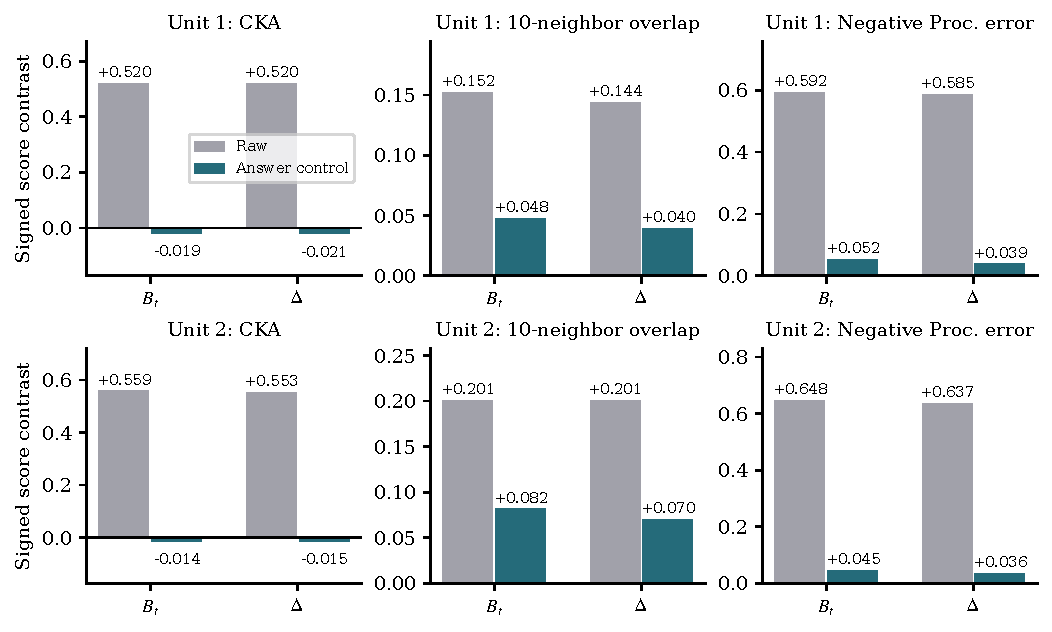
\includegraphics[width=\linewidth]{figures/figure5_matrix_r1.pdf}
\caption{Matrix R1 raw and answer-controlled preferences and increments,
in each of two independent data/initialization units. Control changes the
direction of the aggregated CKA contrast, while the other two controlled
readouts remain positive. Axes are metric-specific; differences of
magnitudes across metrics do not share a common normalization. The example is one relation
in two units and is not a general cross-system law. Original numerical
verification failures on a separate output-probability kNN subset remain
reported in Appendix~\ref{app:verification}.}
\label{fig:matrixcase}
\end{figure}

\section{Discussion and implications for similarity-based arguments}
The observations support a conditional relationship between exact task
correspondences and geometric pairing preferences. In PermWorld the
designated specialist often exceeds a task-candidate mean and frequently
ranks first. The same complete grid also contains negative preferences,
increment reversals, and layer-dependent readings. The graph and matrix
studies further show that answer control and metric choice can change the
answer to an otherwise precisely defined comparison.

Three interpretive distinctions are useful. First, a trained preference
describes a trained geometry, whereas an increment describes that geometry
relative to a specified initial reference. Second, preferring a
transformation for a fixed task pair does not uniquely identify the task
pair under a fixed transformation. Third, an answer-controlled geometric
association is not an identified mathematical mechanism. Pair-specific
residualization, model proficiency, output uncertainty, and general state
organization remain plausible contributors. R1 demonstrates a metric and
control discrepancy after successful learning; it does not settle why that
discrepancy occurs.

For practitioners using similarity to argue that models share a structure,
our design suggests four reporting practices:
\begin{enumerate}
\item Show trained selectivity and its actual initialization reference,
including correct and comparator score changes separately.
\item Under the same transformation, retain a full prespecified candidate
task set and distinguish above-average agreement from uniquely identifying
the designated correspondence.
\item Report raw, answer-controlled, and output-reference geometry, together
with group/support changes and undefined measurements.
\item Keep the designated layer primary while showing prescribed layer and
metric sensitivities; disagreements constrain the claim rather than
providing a reason to select a favorable readout.
\end{enumerate}
These practices apply beyond mathematical testbeds whenever representation
similarity is used as evidence about shared task structure. They are a
measurement discipline; the present experiments do not establish that every
application will show the same positive preferences.

\section{Limitations}
\label{sec:limitations}
\paragraph{Shared initials and limited independent replication.}
The principal PermWorld result uses one data world and one actual
initialization per architecture, copied across specialists and encodings.
GraphWorld reuses the Transformer initial. Shared weights make
Eq.~\ref{eq:initialnull} interpretable, but do not show that the same
preferences hold when specialist initializations are independent, or across
new PermWorld data/initial units. This is the foremost replication gap.
The two matrix worlds independently vary data and initialization together;
they do not isolate the effect of initialization and do not confirm the
PermWorld 32-condition count. Independent paired worlds and independently
initialized specialists would answer different follow-up questions.

\paragraph{Configuration, proficiency, and encoding.}
Transformer and GRU capacities differ, so their comparison is between the
declared configurations rather than a pure architecture effect. Several
cycle-encoding or matrix-XOR tasks remain weak. We retain their scores and
training-defined modal baselines instead of requiring favorable geometry
or a post hoc accuracy threshold. Exceeding a length mode does not imply
full task mastery, and low aggregate accuracy does not prove that a model
ignores all input content. The high-proficiency GRU example and R1 constrain
a universal learning-failure account but do not remove proficiency
confounding elsewhere. Matching updates and example exposures also does not
match FLOPs, wall time, or the number of input tokens processed. Encoding
changes tokenization and positions;
the present intervention does not separate every component of encoding.

\paragraph{Control support, dependency, and sampling.}
Answer residualization varies by candidate and does not remove all nonlinear
label or confidence information. Wrong transformations have accidental
answer matches. Tasks share inputs, weights, schedules, and transformation
families, and the eight permutation relations are not eight independent
scientific replications. We report deterministic summaries on the fixed
analysis samples without inference treating pairs, lengths, metrics, or
conditions as independent draws. Orbit rejection and graph-density mixtures
also restrict the sampled distributions. Counts from different systems
cannot be pooled into a cross-domain effect.

\paragraph{Measurement and mechanism.}
CKA, neighbor overlap, and Procrustes emphasize different geometry and have
different invariances. Gold-answer controls are informative but are not an
input-deconfounding or causal-identification theorem. The study does not
establish transfer gains, infer unobserved composite relations, or identify
a group-specific internal computation. Matrix row/column identities also
hold for general binary matrices and resemble graph-degree relationships.
Transpose is an anti-automorphism, while multiplication by a fixed
invertible matrix is an action; neither result demonstrates learned group
multiplication. Original output-neighbor numerical failures remain a
reported reproducibility limitation, not repaired by the paper's wording.

\section{Conclusion}
Exact mathematical task correspondences are often associated with
representation pairing selectivity in the measured settings. What is
selected, and what changed through training, depend on the comparison,
initial reference, encoding, layer, and control. A raw fixed-transform
candidate comparison provides a particularly clear training-origin
reference under shared initial weights; answer stratification changes that
reference. The full task grid and the matrix $F_1/F_2$ transpose example
with perfect measured task accuracy show why
one positive score is insufficient to identify a shared mathematical
mechanism. The practical contribution is to make these distinctions explicit
and reproducible while retaining their empirical boundaries.

\bibliography{references}
\bibliographystyle{tmlr}

\appendix
\section{Exact task relationships}
\label{app:relations}
For a permutation of $[n]$, let $C(\pi)(i)=n+1-\pi(i)$ and
$I(\pi)=\pi^{-1}$. Table~\ref{tab:relations} records the full declared
catalogue, in its original order. A component is a direct-sum component;
a global descent separates an initial segment whose values all exceed the
remaining values. The offset in P8 is part of the exact formula, not a
change of numeric task labels. The wrong action is complement for the two
inverse relations and inverse for the six complement relations. Identity
pairing is also retained for every relation.

\begin{table}[h]
\centering\small
\begin{tabular}{llll}
\toprule
ID & Left task $f$ & Right task $g_*$ & Exact identity\\
\midrule
P1 & Descents & Recoils (inverse descents) & $f(\pi)=g_*(I\pi)$\\
P2 & Peaks & Valleys & $f(\pi)=g_*(C\pi)$\\
P3 & Fixed points & Anti-fixed points & $f(\pi)=g_*(C\pi)$\\
P4 & Exceedances & Deficiencies & $f(\pi)=g_*(I\pi)$\\
P5 & LIS length & LDS length & $f(\pi)=g_*(C\pi)$\\
P6 & Longest increasing run & Longest decreasing run & $f(\pi)=g_*(C\pi)$\\
P7 & Left-to-right maxima & Left-to-right minima & $f(\pi)=g_*(C\pi)$\\
P8 & Global descents & Components & $f(\pi)=g_*(C\pi)-1$\\
\bottomrule
\end{tabular}
\caption{All eight directed PermWorld relationships. Tasks are defined by
the frozen exact registry; the relationship ID is used in the full tables
and figures. Complement-related instances share a transformation family.}
\label{tab:relations}
\end{table}

GraphWorld uses loop-free directed adjacency matrices $A$. Reversal is
$R(A)=A^\top$ and complement is $C(A)=J-I-A$. Thus maximum out-degree
becomes maximum in-degree under $R$, likewise for minimum degree; maximum
out- or in-degree becomes $n-1$ minus the respective minimum under $C$.
These are four directed instances from two transformation types. Define the
fixed wrong comparator $W$ by shuffling the lexicographically ordered
unordered vertex pairs with the recorded seed $20261010+n$, swapping
successive pairs, and preserving the orientation of their two directed
edges. If one pair remains, it stays fixed. The wrong actions are $W\circ R$
and $W\circ C$. The source release includes their exact mapping and
per-anchor formula-match Booleans. Graphs are drawn from an off-diagonal
Bernoulli mixture with $p\in\{0.25,0.5,0.75\}$, subject to disjoint
$\langle R,C,W\rangle$ split orbits. A fixed position-wise binary one-hot
input kernel is isometric under these slot/category operations and cannot
distinguish correct and wrong pairings. This is one static input reference,
not a claim that every input feature map has identical geometry.

In MatrixGroupWorld, all matrix arithmetic is over $\Ftwo$, while $\wt$
counts nonzero bits as an ordinary integer. Define
\[
 F_1(A)=\wt(Ae_1),\quad F_2(A)=\wt(A^\top e_1),\quad
 F_3(A)=\wt(A(e_1+e_2)),\quad F_4(A)=\wt(A^\top(e_1+e_2)).
\]
With $Q=I+E_{21}$ and $P$ swapping coordinates 1 and 2, the original
catalogue is
\begin{center}\small
\begin{tabular}{llll}
\toprule
Relation & Directed tasks & Correct $T(A)$ & Wrong $U(A)$\\
\midrule
R1 (primary) & $F_1\to F_2$ & $A^\top$ & $PA^\top$\\
R2 (supplementary) & $F_3\to F_4$ & $A^\top$ & $Q^\top A^\top$\\
R3 (primary) & $F_1\to F_3$ & $AQ$ & $AQ^\top$\\
R4 (supplementary) & $F_2\to F_4$ & $Q^\top A$ & $QA$\\
\bottomrule
\end{tabular}
\end{center}
Each correct action satisfies $g_*(T(A))=f(A)$. These identities require
neither uniform sampling over $\mathrm{GL}(n,\Ftwo)$ nor a learned group
representation. The embedded left/right $\mathrm{GL}(2,\Ftwo)$ actions,
with transpose, yield at most 72 orbit members for split exclusion.

\section{Complete primary PermWorld decomposition}
\label{app:fullperm}
Table~\ref{tab:allperm} gives all 32 primary conditions. The companion CSV
preserves full floating-point precision. There is no omitted negative
condition and no inference using the 32 rows as independent repetitions.

\begin{table}[h]
\centering\scriptsize
\setlength{\tabcolsep}{3.0pt}
\begin{tabular}{llrrrrrrrrr}
\toprule
& & $S_c^0$ & $S_u^0$ & $S_c^t$ & $S_u^t$ & $B_0$ & $B_t$ & $\delta_c$ & $\delta_u$ & $\Delta$\\
\midrule
P1 & TF / line & $+0.066$ & $+0.671$ & $+0.119$ & $+0.026$ & $-0.605$ & $+0.093$ & $+0.053$ & $-0.645$ & $+0.698$ \\
P1 & TF / cycle & $+0.812$ & $+0.027$ & $+0.047$ & $+0.079$ & $+0.785$ & $-0.032$ & $-0.765$ & $+0.052$ & $-0.817$ \\
P1 & GRU / line & $+0.079$ & $+0.696$ & $+0.103$ & $+0.036$ & $-0.617$ & $+0.068$ & $+0.024$ & $-0.660$ & $+0.684$ \\
P1 & GRU / cycle & $+0.817$ & $+0.016$ & $+0.109$ & $+0.030$ & $+0.801$ & $+0.079$ & $-0.708$ & $+0.014$ & $-0.722$ \\
P2 & TF / line & $+0.672$ & $+0.072$ & $+0.350$ & $+0.012$ & $+0.600$ & $+0.338$ & $-0.322$ & $-0.060$ & $-0.262$ \\
P2 & TF / cycle & $+0.028$ & $+0.808$ & $+0.067$ & $+0.010$ & $-0.780$ & $+0.057$ & $+0.039$ & $-0.798$ & $+0.837$ \\
P2 & GRU / line & $+0.698$ & $+0.081$ & $+0.886$ & $+0.012$ & $+0.617$ & $+0.874$ & $+0.188$ & $-0.069$ & $+0.257$ \\
P2 & GRU / cycle & $+0.017$ & $+0.816$ & $+0.527$ & $+0.012$ & $-0.799$ & $+0.514$ & $+0.510$ & $-0.803$ & $+1.313$ \\
P3 & TF / line & $+0.670$ & $+0.059$ & $+0.091$ & $+0.011$ & $+0.611$ & $+0.080$ & $-0.580$ & $-0.048$ & $-0.531$ \\
P3 & TF / cycle & $+0.040$ & $+0.661$ & $+0.013$ & $+0.014$ & $-0.622$ & $-0.002$ & $-0.027$ & $-0.647$ & $+0.620$ \\
P3 & GRU / line & $+0.697$ & $+0.072$ & $+0.107$ & $+0.024$ & $+0.624$ & $+0.083$ & $-0.590$ & $-0.048$ & $-0.542$ \\
P3 & GRU / cycle & $+0.028$ & $+0.516$ & $+0.014$ & $+0.026$ & $-0.487$ & $-0.012$ & $-0.014$ & $-0.490$ & $+0.475$ \\
P4 & TF / line & $+0.067$ & $+0.676$ & $+0.129$ & $+0.037$ & $-0.610$ & $+0.092$ & $+0.062$ & $-0.639$ & $+0.701$ \\
P4 & TF / cycle & $+0.650$ & $+0.039$ & $+0.128$ & $+0.011$ & $+0.612$ & $+0.117$ & $-0.522$ & $-0.028$ & $-0.494$ \\
P4 & GRU / line & $+0.080$ & $+0.703$ & $+0.177$ & $+0.132$ & $-0.623$ & $+0.045$ & $+0.097$ & $-0.571$ & $+0.669$ \\
P4 & GRU / cycle & $+0.499$ & $+0.028$ & $+0.131$ & $+0.021$ & $+0.471$ & $+0.110$ & $-0.369$ & $-0.007$ & $-0.361$ \\
P5 & TF / line & $+0.671$ & $+0.049$ & $+0.216$ & $+0.036$ & $+0.622$ & $+0.180$ & $-0.455$ & $-0.013$ & $-0.442$ \\
P5 & TF / cycle & $+0.027$ & $+0.807$ & $+0.130$ & $+0.081$ & $-0.780$ & $+0.049$ & $+0.104$ & $-0.726$ & $+0.829$ \\
P5 & GRU / line & $+0.698$ & $+0.067$ & $+0.517$ & $+0.062$ & $+0.631$ & $+0.455$ & $-0.181$ & $-0.005$ & $-0.176$ \\
P5 & GRU / cycle & $+0.016$ & $+0.811$ & $+0.404$ & $+0.161$ & $-0.795$ & $+0.242$ & $+0.388$ & $-0.649$ & $+1.037$ \\
P6 & TF / line & $+0.670$ & $+0.068$ & $+0.394$ & $+0.018$ & $+0.602$ & $+0.376$ & $-0.276$ & $-0.050$ & $-0.226$ \\
P6 & TF / cycle & $+0.027$ & $+0.812$ & $+0.137$ & $+0.010$ & $-0.784$ & $+0.127$ & $+0.110$ & $-0.801$ & $+0.911$ \\
P6 & GRU / line & $+0.696$ & $+0.078$ & $+0.788$ & $+0.013$ & $+0.619$ & $+0.775$ & $+0.092$ & $-0.064$ & $+0.156$ \\
P6 & GRU / cycle & $+0.016$ & $+0.816$ & $+0.033$ & $+0.136$ & $-0.800$ & $-0.104$ & $+0.016$ & $-0.680$ & $+0.696$ \\
P7 & TF / line & $+0.686$ & $+0.051$ & $+0.211$ & $+0.127$ & $+0.634$ & $+0.084$ & $-0.475$ & $+0.076$ & $-0.551$ \\
P7 & TF / cycle & $+0.024$ & $+0.797$ & $+0.110$ & $+0.053$ & $-0.773$ & $+0.056$ & $+0.085$ & $-0.744$ & $+0.829$ \\
P7 & GRU / line & $+0.698$ & $+0.079$ & $+0.487$ & $+0.073$ & $+0.619$ & $+0.414$ & $-0.212$ & $-0.006$ & $-0.205$ \\
P7 & GRU / cycle & $+0.016$ & $+0.815$ & $+0.236$ & $+0.086$ & $-0.799$ & $+0.150$ & $+0.221$ & $-0.729$ & $+0.950$ \\
P8 & TF / line & $+0.674$ & $+0.059$ & $+0.073$ & $+0.019$ & $+0.614$ & $+0.054$ & $-0.601$ & $-0.040$ & $-0.560$ \\
P8 & TF / cycle & $+0.025$ & $+0.790$ & $+0.028$ & $+0.040$ & $-0.765$ & $-0.012$ & $+0.003$ & $-0.750$ & $+0.753$ \\
P8 & GRU / line & $+0.695$ & $+0.075$ & $+0.489$ & $+0.059$ & $+0.620$ & $+0.430$ & $-0.206$ & $-0.016$ & $-0.190$ \\
P8 & GRU / cycle & $+0.015$ & $+0.808$ & $+0.032$ & $+0.163$ & $-0.793$ & $-0.131$ & $+0.017$ & $-0.645$ & $+0.662$ \\
\bottomrule
\end{tabular}

\caption{Joint-answer-controlled, final-normalized ordinary CKA, computed
per length before equal weighting. Values are rounded to three decimals
only for presentation; formulas and exported tables retain full precision.
``Cycle'' means canonical cycle. The original identity pairing and other
controls remain in the public source tables.}
\label{tab:allperm}
\end{table}

\section{Training and additional measurement details}
\label{app:training}
The declared optimization uses AdamW with learning rate $3\times10^{-4}$,
weight decay 0.01, $\beta=(0.9,0.999)$, $\epsilon=10^{-8}$,
1,000 warmup updates, minimum learning-rate ratio 0.1, and gradient norm
clipping at 1.0. Microbatches of sixteen accumulated four times give an
effective batch of sixty-four. Parameters use FP32 and CUDA BF16 autocast
when available; TF32 is disabled. The vocabulary has 188 tokens and maximum
sequence length is 128. The causal answer-plus-EOS objective supervises two
tokens per example in either permutation encoding.

Balanced random size-permutation blocks determine the saved update
schedule. All specialists within a world use the same sequence of anchor
IDs. Original four-task PermWorld runs retain their recorded task-specific
starting random states; the twelve additional tasks reuse the saved
architecture-specific descents starting state. Encoding pairs share the
exact applicable stream. Thus parameter sharing is exact while a claim
that all sixteen tasks had distinct independent random streams would be
incorrect. Existing source versions and engineering corrections are
individually recorded in the checkpoint receipts.

Each score is evaluated at the logical input end before the task query;
this may be a different absolute token position under the two encodings.
The embedding measurement at this position is not a pooled representation
of all input tokens. All declared intermediate layers are retained for
their prescribed CKA analyses. Static positional/input and gold-answer
references have no fictitious trained-minus-initial increment.

In each comparison, answer means are computed separately on fitting and
held-out strata, according to the original oracle measurement protocol.
Procrustes fitting uses validation data, rank
$\min(8,d_f,d_g)$ when supported, PCA bases and RMS scales estimated on the
fit split, then an orthogonal alignment. A rank-deficient fit is reported
undefined rather than reducing the declared rank to obtain a value.
The score is the negative held-out normalized RMS error, not CKA on
aligned features and not a task-transfer accuracy.

PermWorld and GraphWorld output references use conditional probabilities
over numeric answers 0--30; MatrixGroupWorld retains its original full
188-token output softmax. These distinct baseline constructions are not
pooled as a common cross-system effect. Source answer accuracy is reported
over the full vocabulary. Length/size mode baselines use training labels
with the original smallest-label tie rule, rather than fitting a test-set
mode. The public tables include the per-size values and source learning
scores, including weak specialists and undefined baseline measurements.

\section{Numerical verification and source availability}
\label{app:verification}
MatrixGroupWorld retains its original
\texttt{completed\_with\_verification\_caveat} status:
eight actual 20k endpoints, numerical status counts 64 passed, 2 failed,
and 6 \texttt{undefined\_consistent}, with
\texttt{scientific\_analysis\_complete=false}. Both failures concern the
trained raw \emph{output-probability} kNN score in unit 1, R1, $n=6$, on
the fixed 64-input subset. The production and independent values differ
by $1/640$: $0.600000$ versus $0.6015625$ for the correct view and
$0.1656250$ versus $0.1671875$ for the wrong view. Both exceed the original
$10^{-8}$ tolerance. A read-only diagnosis localizes near-onehot distance
roundoff without changing the metric, values, tolerance, or failed status.
Those two failed records concern output probabilities. The hidden-CKA
checks on the fixed subset record no failures; the audit does not
independently verify all 432 production cells.

Code, complete tables, protocols, checkpoint/source identities, and actual
data and array packages are available at
\url{https://github.com/XuanyuYang223/2026TMLR} and its
representation-selectivity artifact release. The paper reads saved tables
at publication/saved-table snapshot \texttt{d9a113d}; actual execution
versions remain recorded separately in the source receipts. Its figures are reproducible with the
companion CSV-only plotting script. The publisher separately verified all
89 local archive streams and member SHAs and all public provider sizes and
digests. A fresh public clone actually downloaded thirteen artifact
packages and independently checked the main saved-table aggregates. These
are engineering and arithmetic checks, not new statistical replications or
full model-forward reproductions. Historical constructor-rebuilt or
unverified initials are kept separate from the genuine initials used in
the primary study. Seven historical pre-repair source revisions remain
unavailable; no exact replay of every historical development state is
claimed.

The additional workshop bibliography item remains a draft task pending
verified title/author/venue information. Before a formal anonymous
submission, author-identifying repository links should be handled according
to the chosen submission policy. This document is publicly shared as a
working draft and has not been formally submitted for publication.

\end{document}
